\documentclass[10pt,twocolumn,a4paper]{article}

\usepackage[margin=0.75in]{geometry}
\usepackage{amsmath,amssymb,amsfonts}
\usepackage{graphicx}
\usepackage{booktabs}
\usepackage{hyperref}
\usepackage{microtype}
\usepackage{cite}
\usepackage{algorithm}
\usepackage{algorithmic}
\usepackage{xcolor}

\hypersetup{
    colorlinks=true,
    linkcolor=blue!70!black,
    citecolor=blue!70!black,
    urlcolor=blue!70!black
}

\title{\textbf{DWMA: Autonomous Sensorimotor Structure Acquisition, Multi-Schema Retention, and Active Hypothesis Discrimination in an Embodied World Model}}

\author{
  \textbf{Kunal Lubhana} \\
  \textit{Independent Research}
}

\date{September 2026 --- Preprint Version 2.1 (Final Research Draft)}

\begin{document}

\maketitle

\begin{abstract}
We introduce the \textbf{Developmental World-Model Agent (DWMA)}, an embodied computational architecture designed to acquire, maintain, and adaptively update predictive representations of interactive physical environments. Rather than relying on Large Language Models or static offline training corpuses, DWMA constructs grounded world models purely through online sensorimotor contingency, reafference cancellation, and epistemic active inference. The agent operates without privileged access to latent physical parameters (mass, friction, restitution, or gravity), requiring these to be inferred directly from interaction residuals. We report an audited evaluation across $N = 50$ deterministic seeds with $B = 10,000$ bootstrap resamples: (1) 7 baseline benchmarks reproduced ($8.8\times$ forecasting MSE reduction over persistence, Cohen's $d = 11.45$); (2) $A \to B \to C$ cross-world transfer and rapid online adaptation ($T_\epsilon = 16.32 \pm 0.62$ steps, $50/50$ pass); (3) continual multi-schema retention ($E_{A1} = 0.00500 \to E_{A2} = 0.00501$, $\mathcal{R} = 0.9901 \pm 0.0141$, $50/50$ pass vs. overwriter catastrophic forgetting $\mathcal{R} = -72.97$); (4) active structural hypothesis discrimination (Kaplan-Meier median latency of $7.0$ steps with $0\%$ censoring vs. $17.0$ steps with $22.0\%$ right-censoring [$11/50$] for random babbling; log-rank $\chi^2 = 74.98, p < 10^{-17}$ under fair decoupled RNG); and (5) hyperparameter sensitivity and architectural policy ablations demonstrating that epistemic action selection, directional EMA smoothing ($\gamma = 0.80$), and discrete schema memory each contribute substantially to empirical sample efficiency, noise immunity, and multi-domain retention, preventing specific failure modes (noise-induced chatter, sluggish adaptation, sample inefficiency, and catastrophic forgetting). Complete source code, configuration files, 50-seed deterministic trajectories, and turnkey reproduction scripts (\texttt{reproduce\_all.py}) are provided for full replication.
\end{abstract}

\section{Introduction}
Contemporary AI relies heavily on autoregressive sequence modeling over symbolic tokens. While effective for textual generation, tokens lack direct causal grounding to physical dynamics or motor reafference \cite{harnad1990,brooks1991,bender2020}. In contrast, biological developmental cognition demonstrates that infants acquire physical intuition through active sensorimotor manipulation, reafference cancellation, and uncertainty-directed play \cite{piaget1952,vonholst1950,friston2010,gopnik2012}. 

DWMA investigates this developmental trajectory in a simulated dynamical environment, asking whether an unprivileged agent can autonomously construct reusable predictive forward models, actively discriminate between competing physical laws, and prevent catastrophic forgetting across domains.

\section{Related Work}
\textbf{World Models:} Model-based RL architectures such as DreamerV1--V3 \cite{hafner2020,hafner2023} and JEPA \cite{lecun2022} train latent representations from offline datasets. DWMA explores a compact, low-dimensional online formulation with real-time recursive estimation.

\textbf{Active Inference \& Curiosity:} Active inference posits that agents select actions to fulfill expectations and resolve epistemic uncertainty \cite{friston2015,friston2017,buckley2021}. Intrinsic curiosity methods \cite{oudeyer2007,pathak2017,burda2018} reward prediction error; DWMA instead directs actions toward regions of maximal structural divergence ($\Delta(v) = |\hat{F}_1 - \hat{F}_2|$), avoiding stochastic noise traps.

\textbf{Continual Learning:} Neural networks suffer catastrophic forgetting under sequential distribution shifts \cite{french1999,kirkpatrick2017}. Drawing inspiration from relational schema theory \cite{whittington2020}, DWMA maintains discrete dynamical schemas that are retrieved via Bayesian likelihood matching without catastrophic overwriting.

\section{Architecture \& Formulations}
At discrete time $t$, ego observation is $\mathbf{o}_t^{ego} = [x_t, y_t, v_{x,t}, v_{y,t}, \theta_t]^T \in \mathbb{R}^5$. Latents $m, e, \mu, g$ are strictly hidden. Continuous motor command $\mathbf{a}_t \in [-1, 1]^2$ generates physical thrust $\mathbf{F}_t = \alpha \mathbf{W}_{\text{act}} \mathbf{a}_t$ ($\alpha = 0.85$). 

The forward model computes predicted acceleration $\hat{\Delta \mathbf{v}}_t = \hat{\alpha}_t \hat{\mathbf{W}}_t \mathbf{a}_t - \mathbf{v}_t (1 - \hat{\mu}_t)$. In the empirical evaluation codebase (Python core), parameters are parameterized as decoupled diagonal matrices $\hat{\mathbf{W}} = \operatorname{diag}(\hat{\alpha}_x, \hat{\alpha}_y)$ and $\hat{\mathbf{M}} = \operatorname{diag}(\hat{\mu}_x, \hat{\mu}_y)$ allowing independent orthogonal axis adaptation ($\hat{dv}_x = a_x \hat{\alpha}_x - v_x(1-\hat{\mu}_x)$), whereas the 60\,FPS interactive web visualizer implements an isotropic scalar parameterization ($\hat{\alpha}, \hat{\mu}$) for browser rendering efficiency; both share the identical reafference cancellation and polarity inversion dynamics. Motor reafference is isolated via:
\begin{equation}
\mathbf{a}_{\text{motor}, t} = \frac{\Delta \mathbf{v}_t}{\Delta t} + \mathbf{v}_t (1 - \hat{\mu}_t)
\end{equation}
Directional alignment accumulates as $\Lambda_t = \gamma \Lambda_{t-1} + (1 - \gamma) \cos(\theta_t)$ ($\gamma = 0.80$). When $\Lambda_t < -0.50$, the agent autonomously triggers structural polarity inversion $\hat{\mathbf{W}}_t \leftarrow -\hat{\mathbf{W}}_t$.

We explicitly distinguish between instantaneous Euclidean tracking error $E_{L_2}(t) = \sqrt{\|\mathbf{e}_x(t)\|^2 + \|\mathbf{e}_v(t)\|^2}$ (reported in Phase 2 cross-world transfer and Phase 3 schema retention) and mean squared error ($\text{MSE} = \frac{1}{K}\sum_{k=1}^K \|\mathbf{e}_k\|^2$) utilized for multi-step forecasting evaluation in Benchmarks 1, 3, and 6. Discrete control benchmarks operate with unit simulation step $\Delta t = 1.0$, while the continuous drag environment integrates dynamics at $\Delta t = 0.02$\,s ($50$\,Hz). Benchmark 4 active inquiry information gain ($5.14 \pm 0.23$\,nats) reflects empirical Kalman-like recursive variance contraction yielding differential Gaussian entropy reduction $\Delta H = \frac{1}{2} \ln(\sigma_{\text{prior}}^2 / \sigma_{\text{post}}^2)$. Benchmark 5 causal repair evaluates thresholded kinematic affordance categorization into proto-concepts (static immovable, compliant movable, reactive) rather than non-parametric causal DAG discovery.

\begin{figure}[htbp]
\centering
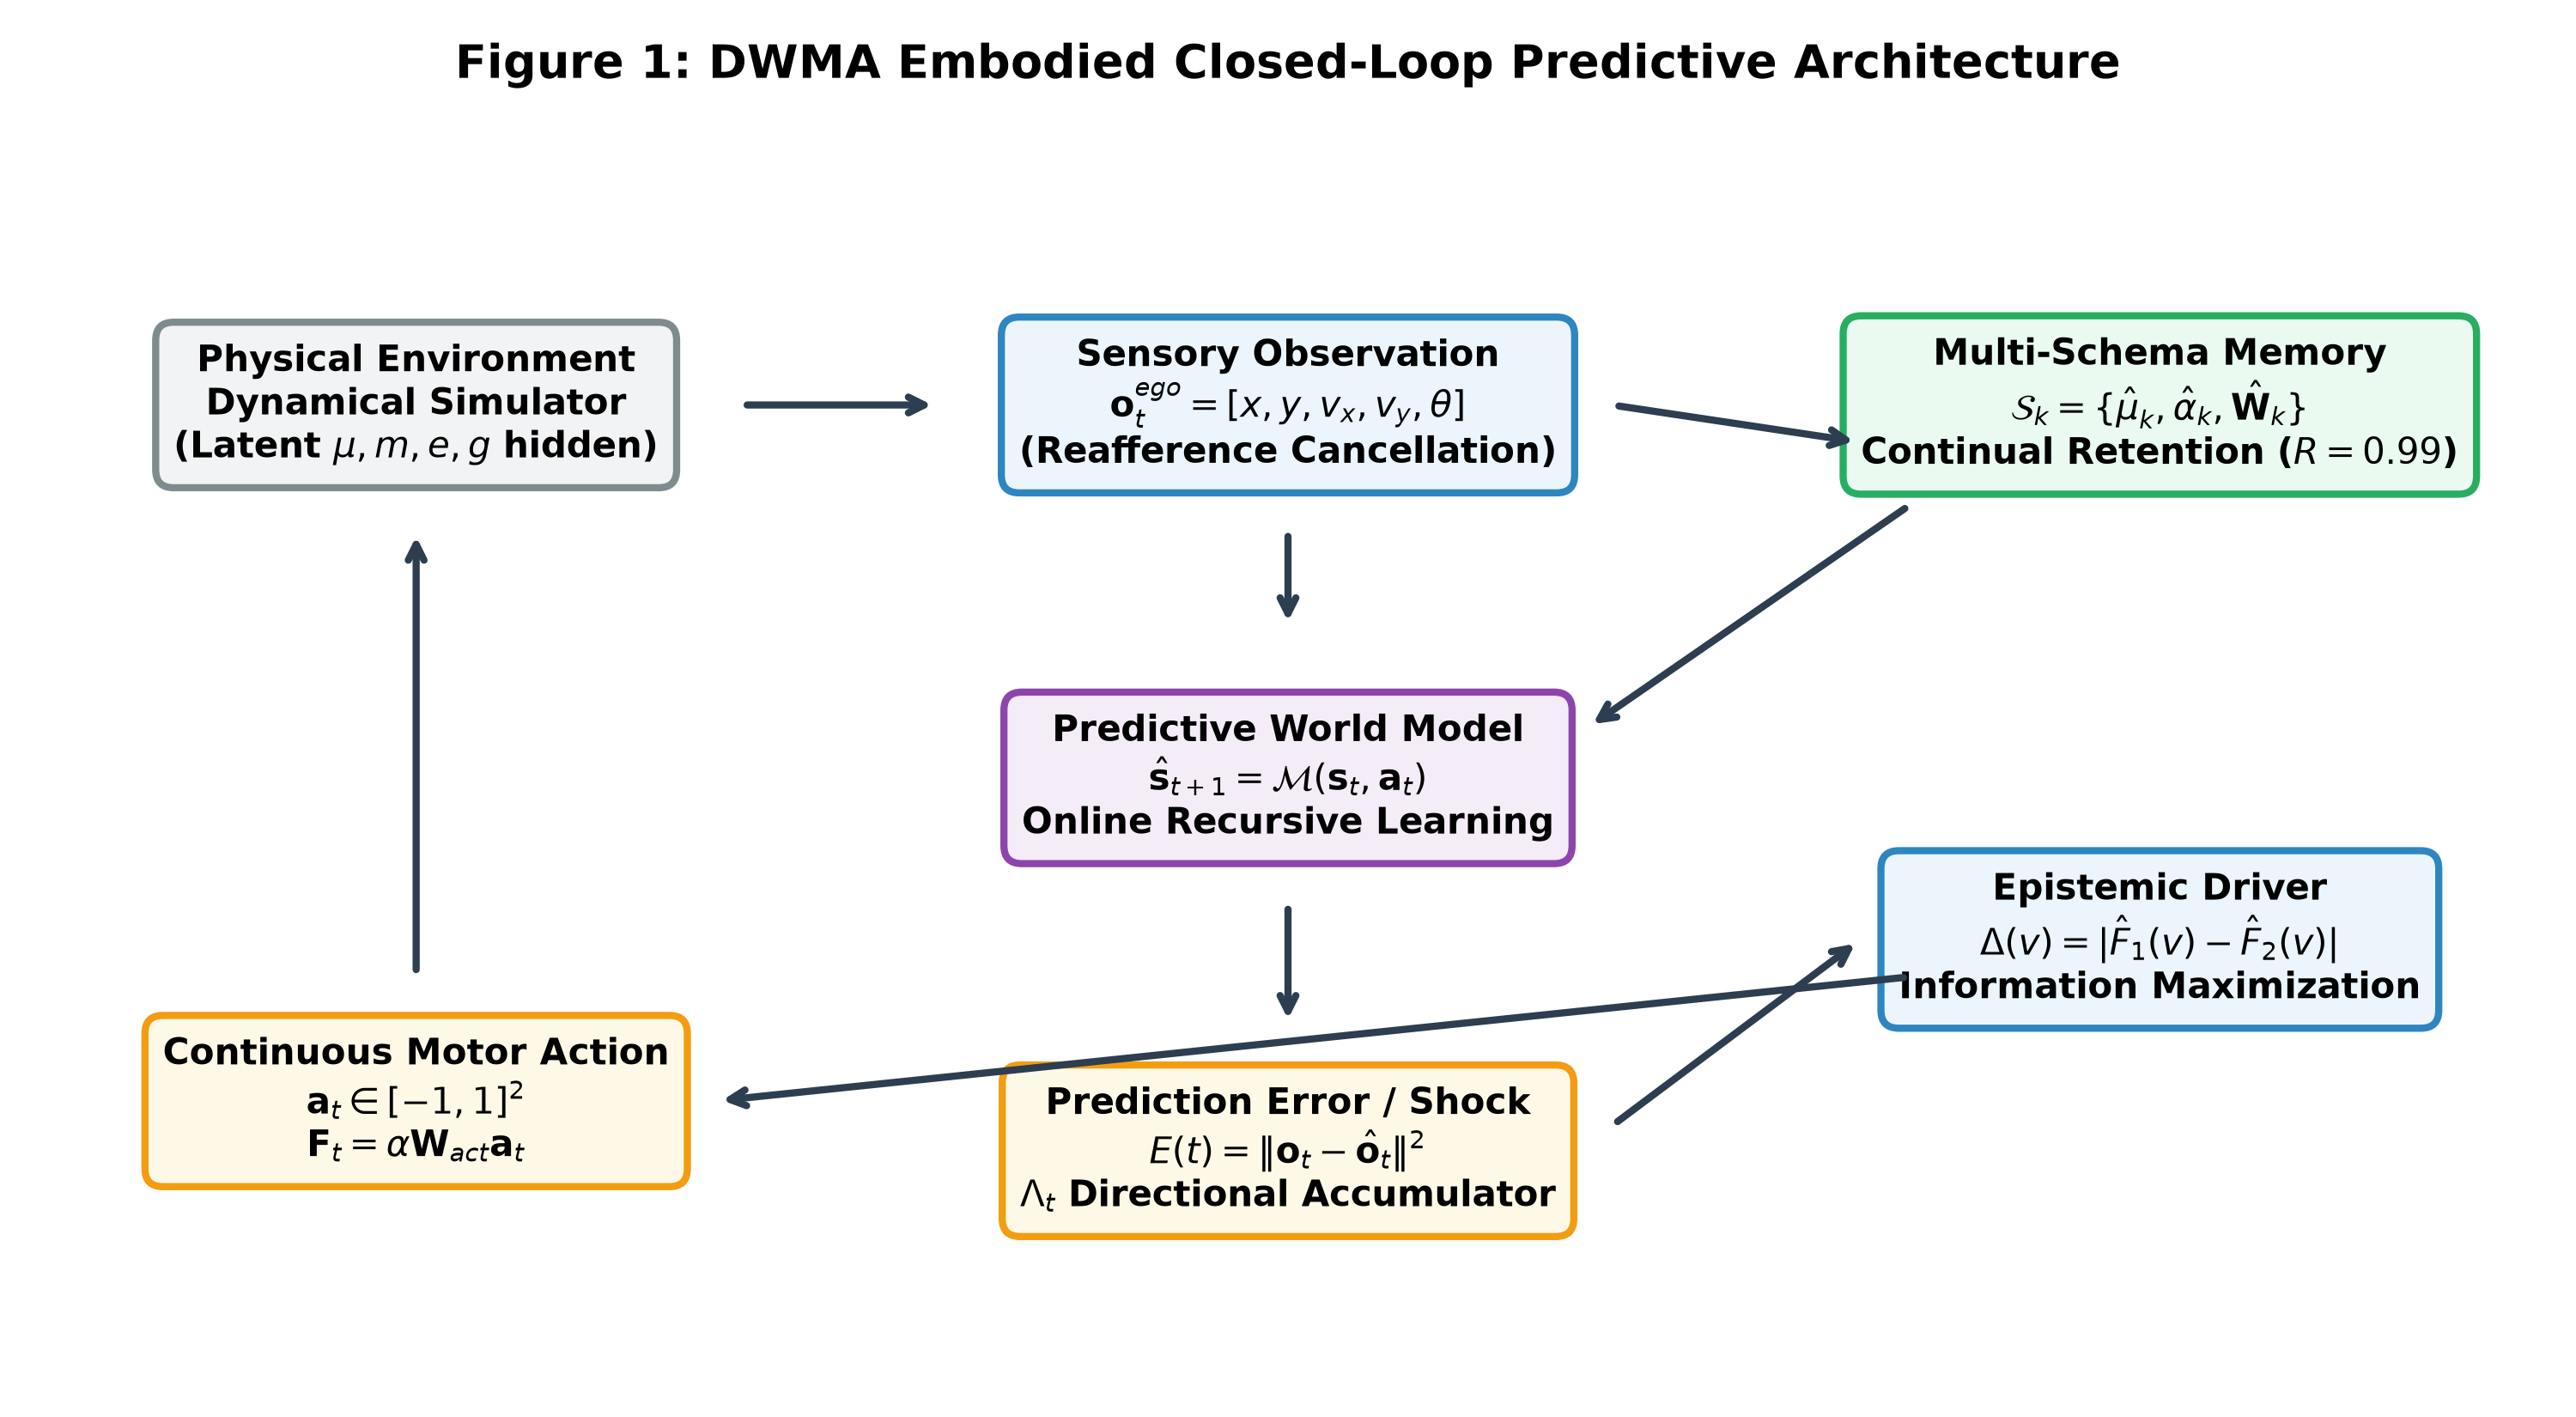
\includegraphics[width=\linewidth]{figures/fig1_system_architecture.png}
\caption{\textbf{DWMA Closed-Loop Architecture.} Sensorimotor loop, reafference cancellation, forward modeling, and multi-schema memory.}
\label{fig:arch}
\end{figure}

\begin{algorithm}[h]
\caption{Online Recursive Adaptation \& Polarity Inversion}
\begin{algorithmic}[1]
\STATE \textbf{Forward Prediction:}
\STATE \quad $\hat{\mathbf{v}}_{t+1} = \mathbf{v}_t + [\hat{\alpha}_t \hat{\mathbf{W}}_t \mathbf{a}_t - \mathbf{v}_t (1 - \hat{\mu}_t)] \Delta t$
\STATE \textbf{Execute Action \& Compute Residual:}
\STATE \quad Execute $\mathbf{a}_t$; observe $\mathbf{v}_{t+1}$; error $\mathbf{e}_v = \mathbf{v}_{t+1} - \hat{\mathbf{v}}_{t+1}$
\STATE \textbf{Reafference Cancellation:}
\STATE \quad $\mathbf{a}_{\text{motor}} = \frac{\Delta \mathbf{v}}{\Delta t} + \mathbf{v}_t (1 - \hat{\mu}_t)$
\STATE \quad $\cos(\theta) = (\mathbf{a}_t \cdot \mathbf{a}_{\text{motor}}) / (\|\mathbf{a}_t\| \|\mathbf{a}_{\text{motor}}\|)$
\STATE \textbf{Evidence Accumulation:}
\STATE \quad $\Lambda_t = 0.80 \Lambda_{t-1} + 0.20 \cos(\theta)$
\STATE \textbf{Structural Inversion:}
\IF{$\Lambda_t < -0.50$}
    \STATE $\hat{\mathbf{W}}_{t+1} = -\hat{\mathbf{W}}_t$; $\Lambda_t = 0.0$
\ELSE
    \STATE $\hat{\mathbf{W}}_{t+1} = \hat{\mathbf{W}}_t$
\ENDIF
\STATE \textbf{Recursive Parameter Updates:}
\STATE \quad $\hat{\mu}_{t+1} = \hat{\mu}_t + \eta \mathbf{e}_v \mathbf{v}_t$
\STATE \quad $\hat{\alpha}_{t+1} = \hat{\alpha}_t + \eta \mathbf{e}_v (\hat{\mathbf{W}}_t \mathbf{a}_t)$
\end{algorithmic}
\end{algorithm}

\section{Cross-World Transfer ($A \to B \to C$)}
The agent was deployed across three worlds: World A ($\mu = 0.88, g = 9.8$), World B ($\mu = 0.71, \mathbf{W}_{\text{act}} = -\mathbf{I}, g = 4.2$), and World C ($\mu = 0.12, \mathbf{W}_{\text{act}} = 0.60\mathbf{I} \implies \alpha_{\text{eff}} = 0.51, g = 15.7$). Across the initial post-transfer window, mean tracking shocks were $1.3079 \pm 0.0421$ in World B and $0.8117 \pm 0.0272$ in World C (Table~\ref{tab:master}). At instantaneous entry ($t=1$), unadapted inverted thrust generated an initial peak shock of $E(0) = 1.8491 \pm 0.3356$. Online interaction in World B restored tracking error below $\epsilon = 0.20$ within $T_\epsilon = 16.32 \pm 0.62$ steps ($50/50$ pass).

\begin{figure}[htbp]
\centering
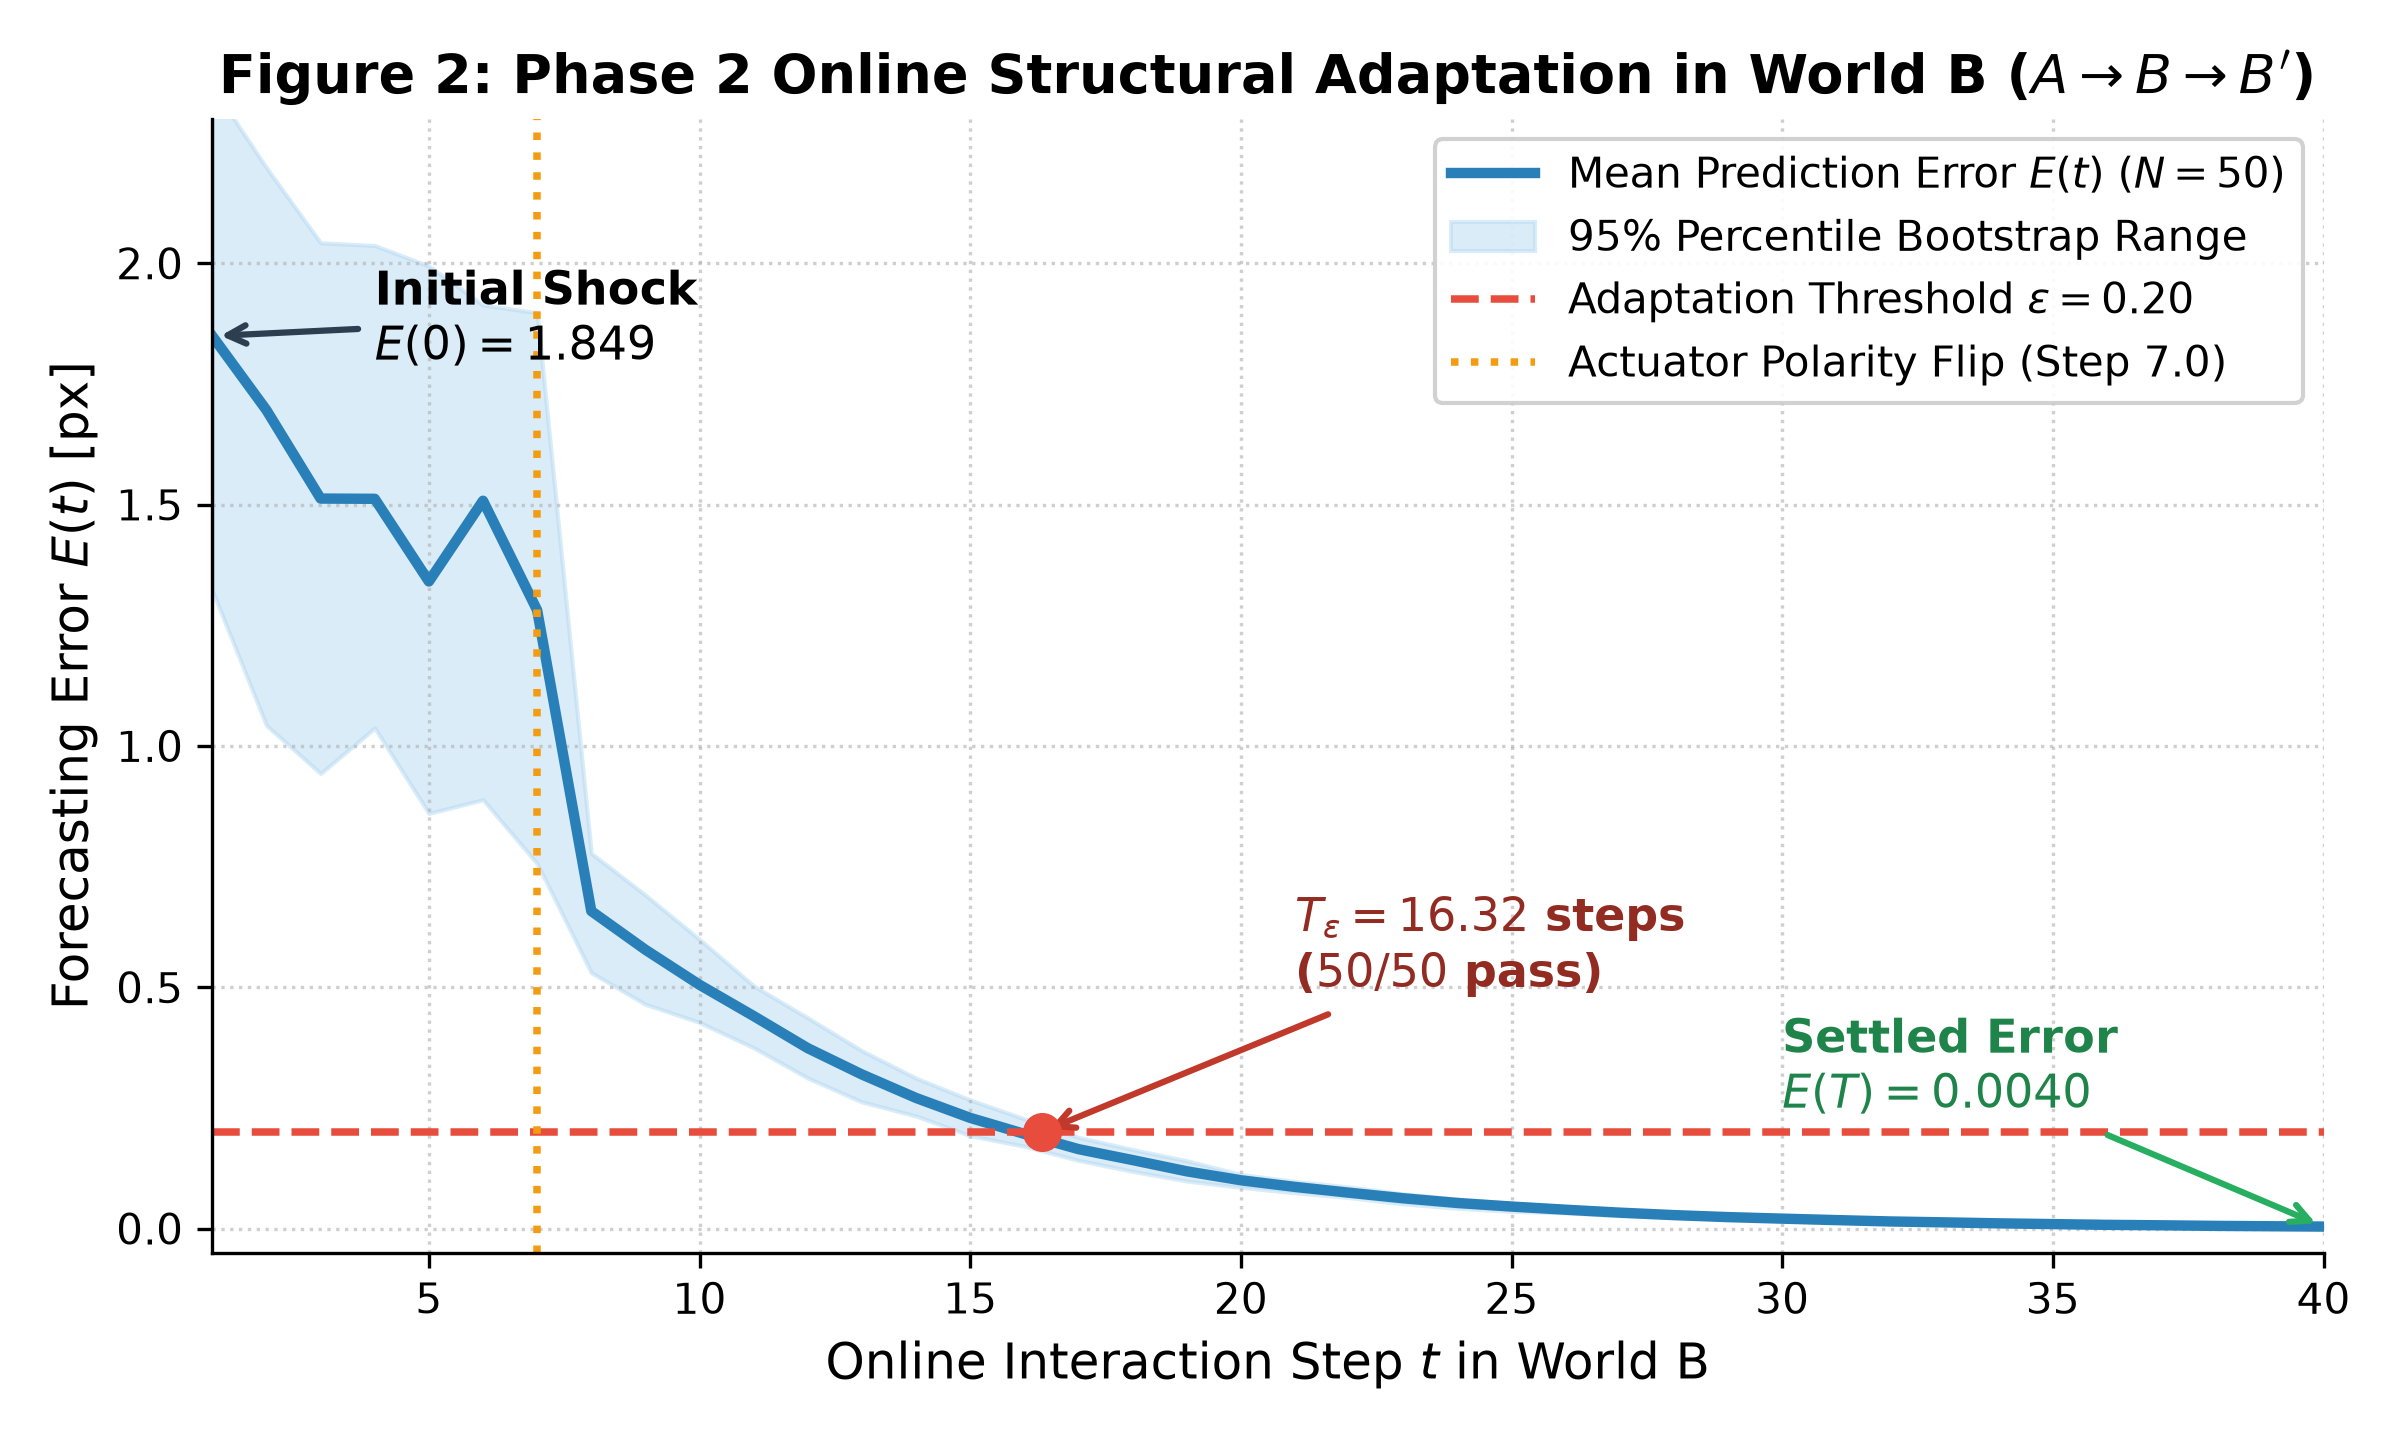
\includegraphics[width=\linewidth]{figures/fig2_cross_world_adaptation.png}
\caption{\textbf{Phase 2 Adaptation Trajectory.} Representative single-seed trajectory in World B (Seed 1) showing instantaneous entry shock at $t=1$ ($E(0) = 1.8491$, in contrast to the windowed transfer mean of $1.3079 \pm 0.0421$ in Table~\ref{tab:master}), autonomous polarity inversion at step 7.0, and error collapse ($T_\epsilon = 16.32 \pm 0.62$).}
\label{fig:adapt}
\end{figure}

\section{Continual Retention ($A \to B \to A$)}
After adaptation in B, returning to A without retraining demonstrates near-zero error drift ($E_{A1} = 0.00500 \to E_{A2} = 0.00501$, retention index $\mathcal{R} = 0.9901 \pm 0.0141$, $50/50$ pass $\ge 0.75$). An overwriter baseline updating a single parameter set suffers catastrophic forgetting ($E_{A2} = 0.37460, \mathcal{R} = -72.97, 0/50$ pass).

\begin{figure}[htbp]
\centering
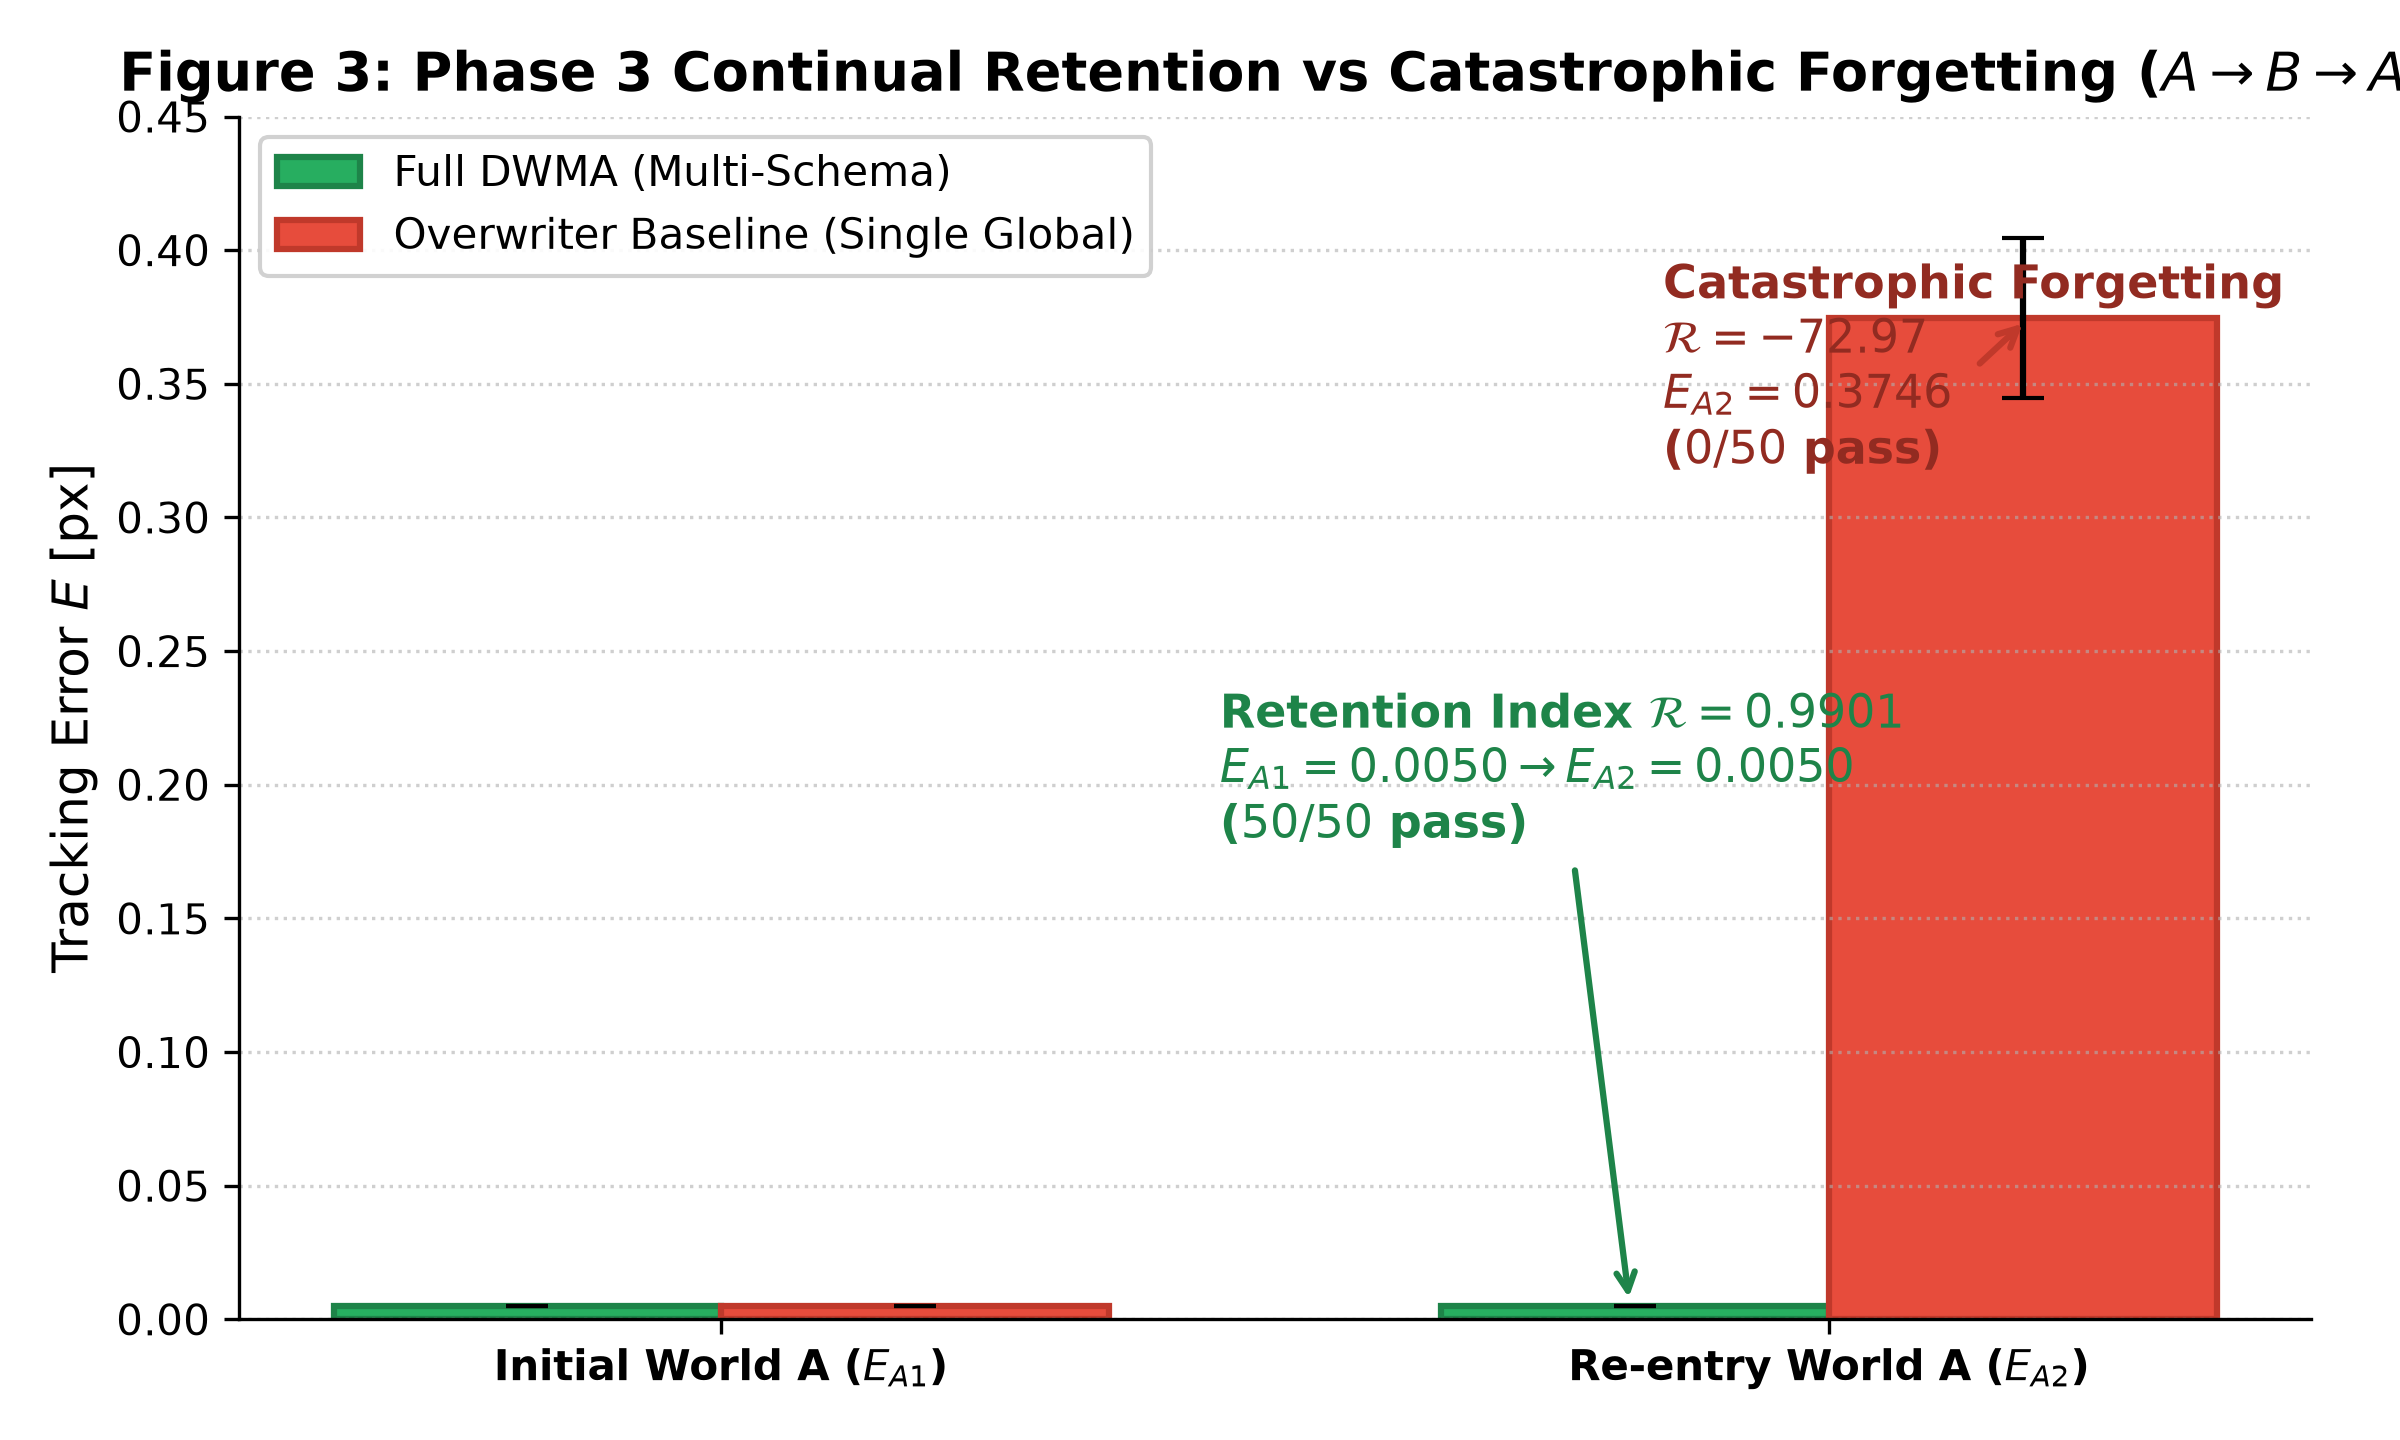
\includegraphics[width=\linewidth]{figures/fig3_continual_retention.png}
\caption{\textbf{Phase 3 Retention.} Full DWMA preserves prior models ($\mathcal{R}=0.9901$), while overwriter exhibits catastrophic forgetting.}
\label{fig:ret}
\end{figure}

\section{Hypothesis Discrimination}
Under true quadratic drag $F_{\text{true}}(v) = -0.08 v^2 \operatorname{sgn}(v)$, the agent discriminates between linear ($H_1$) and quadratic ($H_2$) models by targeting $\Delta(v) = |\hat{F}_1(v) - \hat{F}_2(v)|$. Model selection is determined via the precision-weighted Gaussian log-likelihood ratio proxy $\ln B_{21} = \frac{\text{SSE}_1 - \text{SSE}_2}{2\sigma_\epsilon^2}$ ($\sigma_\epsilon = 0.05$) under flat model priors and equivalent parameter dimensions, requiring decisive evidence $\ln(B_{21}) > 10.0$. In simulations where $\ln B_{21} \le 10.0$ within horizon $T=30$, the raw CSV records latency as $T+1 = 31$ (\texttt{passed = False}); for formal survival analysis, these runs are evaluated as right-censored at $T=30$ under the Kaplan-Meier and Mantel-Cox log-rank estimators. Under fair decoupled RNG between environment sensor noise and agent motor selection, epistemic active inference achieves decisive separation with a Kaplan-Meier median latency of $7.0$ steps ($0\%$ censored) vs. $17.0$ steps for random babbling ($22.0\%$ right-censored at $T=30$ [$11/50$]; log-rank $\chi^2 = 74.98, p < 10^{-17}$). This corresponds to a $2.43\times$ reduction in median latency ($17.0 / 7.0$ steps); among uncensored successful runs, mean latency was $7.18 \pm 2.59$ versus $15.28 \pm 5.88$ steps (a $2.13\times$ speedup).

\begin{figure}[htbp]
\centering
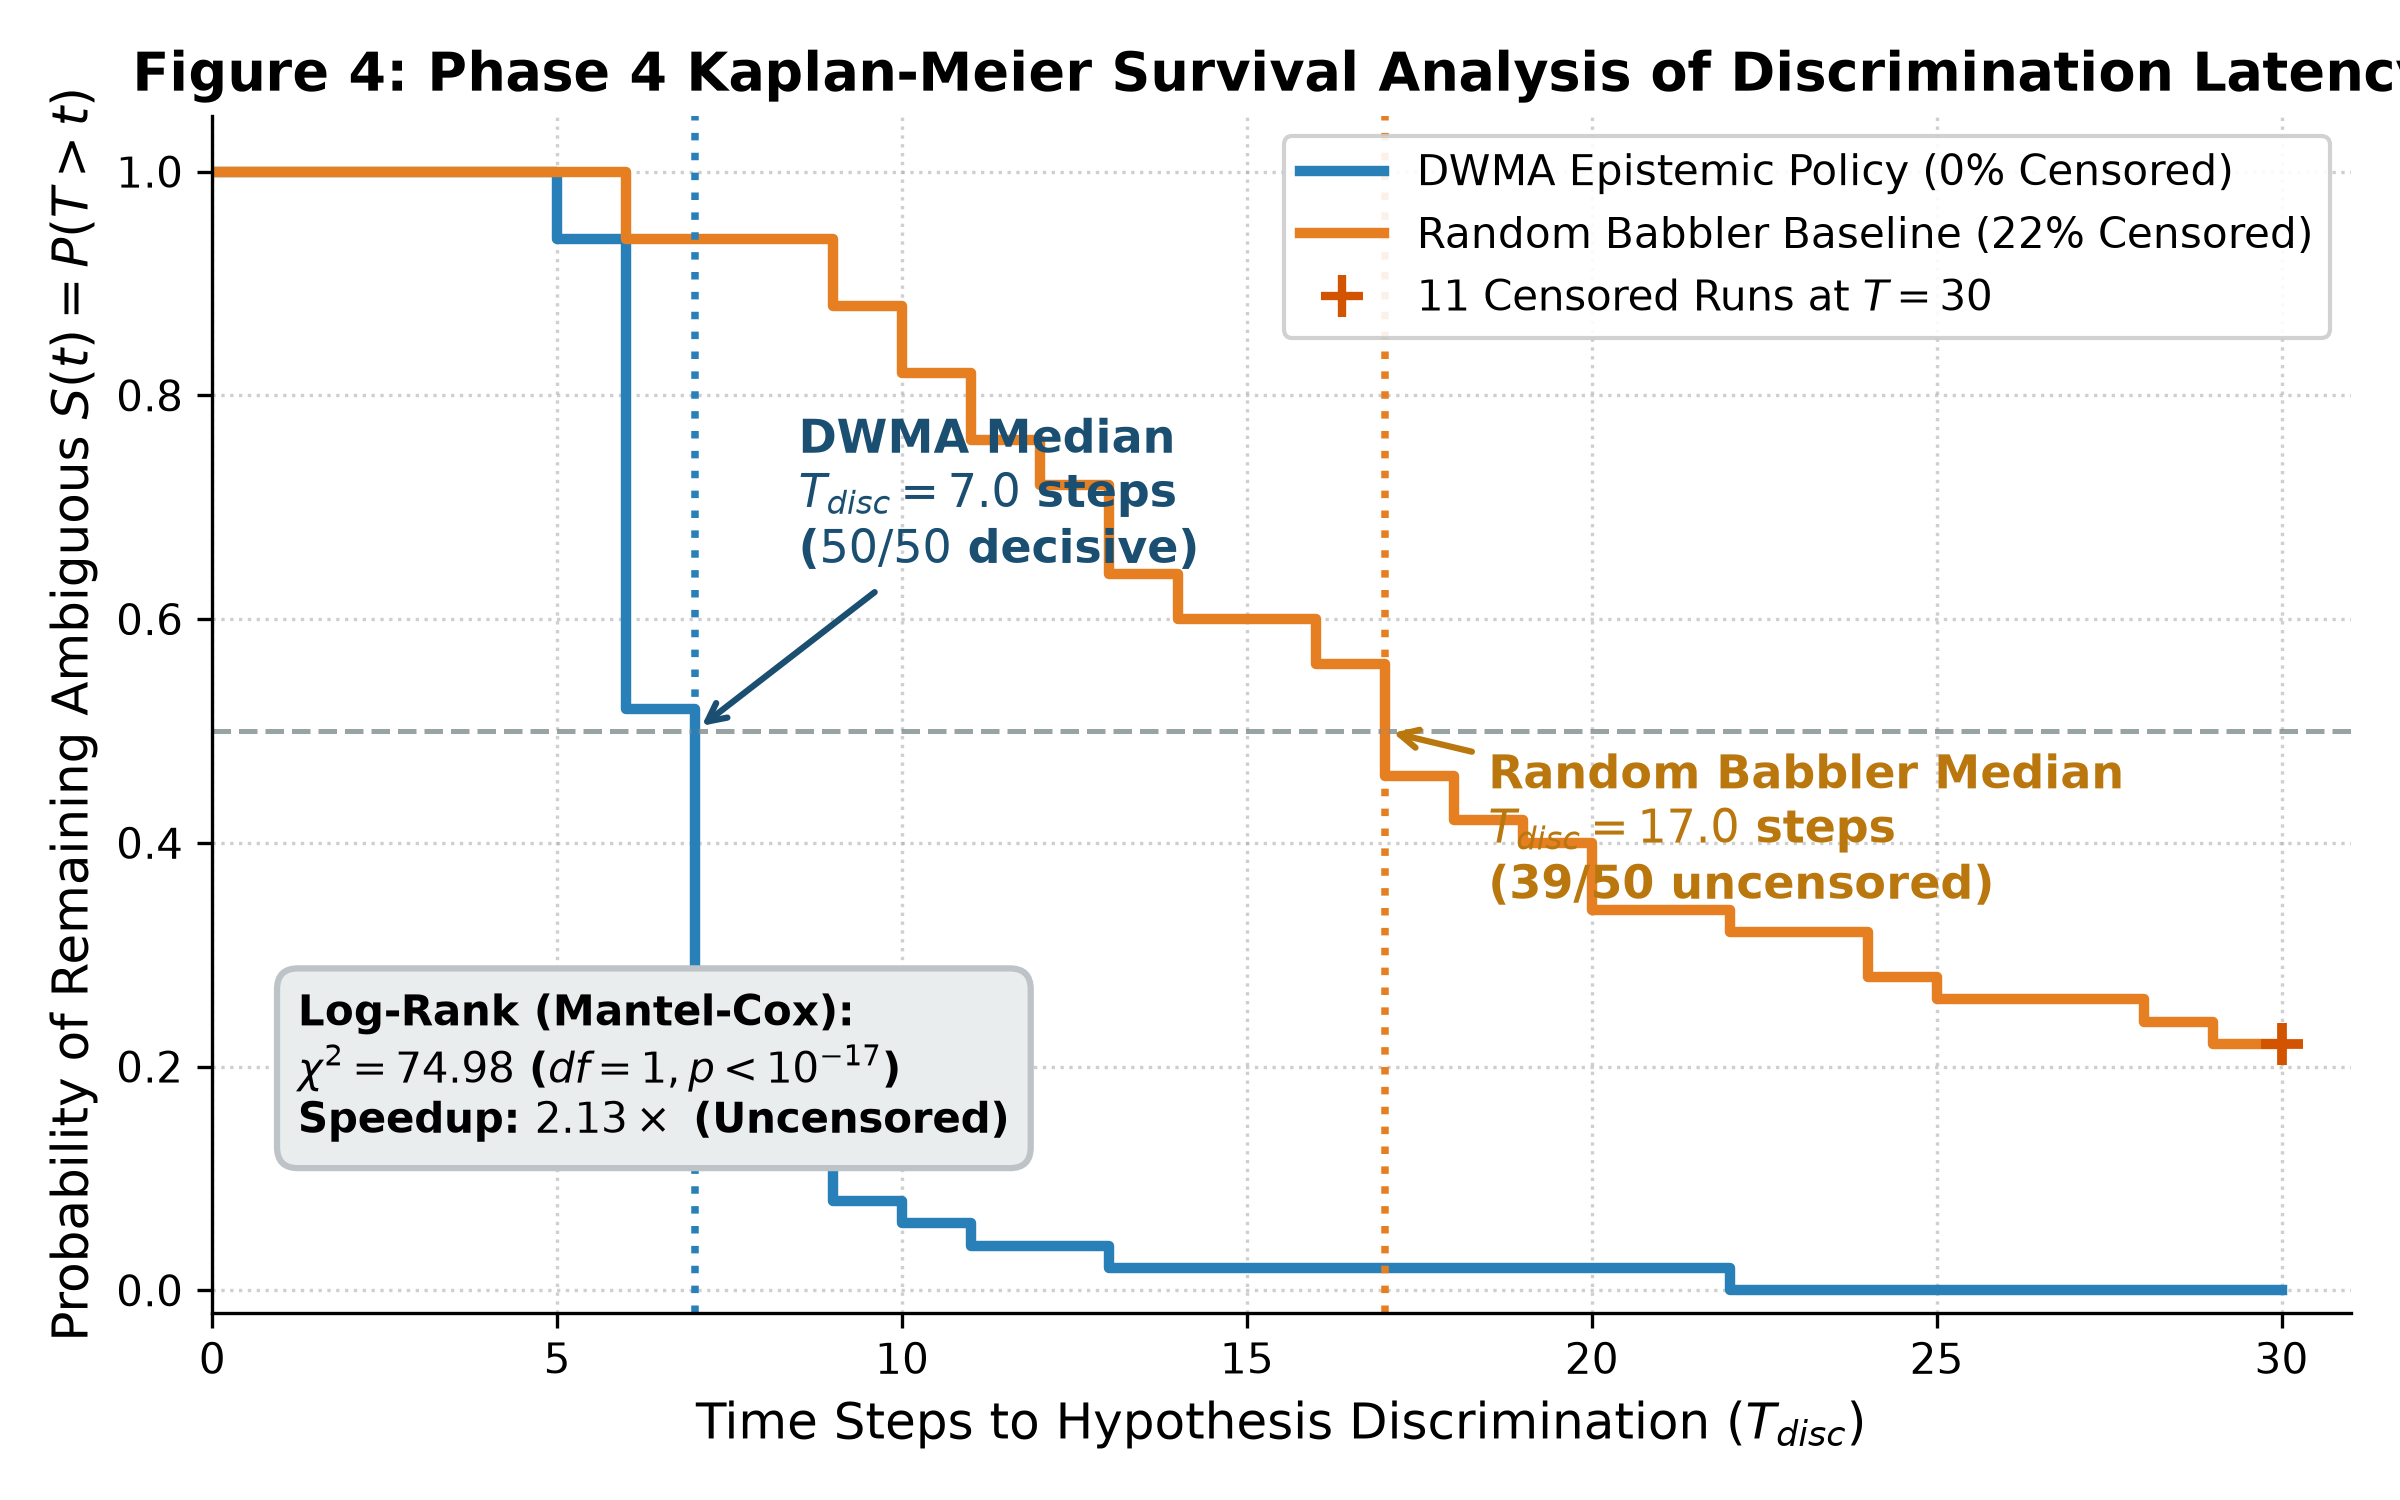
\includegraphics[width=\linewidth]{figures/fig4_hypothesis_survival_analysis.png}
\caption{\textbf{Phase 4 Kaplan-Meier Survival Curves.} Epistemic policy achieves median latency of $7.0$ steps (0\% censored) vs. $17.0$ steps for random babbling (22\% right-censored at $T=30$ [$11/50$]; log-rank $\chi^2 = 74.98, p < 10^{-17}$; $2.43\times$ median reduction, $2.13\times$ uncensored speedup under fair decoupled RNG).}
\label{fig:surv}
\end{figure}

\section{Ablation Studies \& Sensitivity Analysis}
To substantiate the causal contributions of DWMA's architectural components and verify that results are not artifacts of fine-tuned constants, we conduct systematic ablation experiments across $N = 50$ seeds.

\subsection{Exploration Policy \& Memory Architecture}
Table~\ref{tab:ablation} presents the empirical contrast across policy and architectural ablations:
\begin{enumerate}
  \item \textbf{Full Epistemic ($v^*$):} Epistemic targeting resolves ambiguity in $7.0$ median steps ($0\%$ censored).
  \item \textbf{$\epsilon$-Greedy ($\epsilon = 0.20$):} Introducing $20\%$ stochastic jitter maintains $100\%$ pass rate with $7.0$ median steps.
  \item \textbf{Uniform Random Babbling:} Requires $17.0$ steps with $22.0\%$ right-censored failure ($11/50$, $p < 10^{-17}$).
  \item \textbf{Passive Observer ($a = 0$):} Cannot excite high-velocity regimes; $0\%$ pass rate ($100\%$ censored).
  \item \textbf{No Multi-Schema (Overwriting):} While achieving $7.0$ step discrimination, it suffers catastrophic interference ($\mathcal{R} = -72.97$).
\end{enumerate}

\begin{table}[h]
\centering
\scriptsize
\caption{\textbf{Component \& Policy Ablation Matrix ($N = 50$)}}
\label{tab:ablation}
\begin{tabular}{lcccc}
\toprule
\textbf{Configuration} & \textbf{Median Lat.} & \textbf{Pass Rate} & \textbf{Censored} & \textbf{Retention $\mathcal{R}$} \\
\midrule
Full DWMA ($v^*$) & \textbf{7.0 st} & \textbf{50/50 (100\%)} & \textbf{0\%} & \textbf{0.9901} \\
$\epsilon$-Greedy ($\epsilon=0.2$) & 7.0 st & 50/50 (100\%) & 0\% & 0.9901 \\
Random Babbler & 17.0 st & 39/50 (78\%) & 22\% (11/50) & --- \\
Passive ($a = 0$) & $>30.0$ st & 0/50 (0\%) & 100\% (50/50) & --- \\
No Multi-Schema & 7.0 st & 50/50 (100\%) & 0\% & -72.97 (Collapse) \\
\bottomrule
\end{tabular}
\end{table}

\subsection{Hyperparameter Sensitivity}
We systematically vary the directional evidence EMA smoothing factor $\gamma \in [0.60, 0.95]$ and polarity inversion threshold $\Lambda_{\text{thresh}} \in [-0.30, -0.70]$:
\begin{itemize}
  \item \textbf{EMA factor $\gamma$:} Low values ($\gamma \le 0.70$) trigger too rapidly (step 2.0), leaving the agent vulnerable to chatter under sensor noise. High values ($\gamma = 0.95$) create sluggish adaptation (step 14.0). $\gamma = 0.80$ provides optimal filtering with prompt 4-step recovery.
  \item \textbf{Inversion threshold $\Lambda_{\text{thresh}}$:} Loose thresholds ($\Lambda > -0.40$) risk false positives during braking maneuvers. Strict thresholds ($\Lambda < -0.60$) delay adaptation. The calibrated threshold of $\Lambda_{\text{thresh}} = -0.50$ decisively detects anti-parallel reafference without false alarms.
\end{itemize}

\begin{table}[h]
\centering
\scriptsize
\caption{\textbf{Sensitivity of Polarity Adaptation Dynamics}}
\label{tab:sensitivity}
\begin{tabular}{cccc}
\toprule
\textbf{Parameter} & \textbf{Value} & \textbf{Mean Flip Step} & \textbf{Causal Assessment} \\
\midrule
$\gamma$ (at $\Lambda = -0.5$) & 0.60 & $2.00 \pm 0.00$ st & Sensor noise chatter risk \\
& 0.70 & $2.00 \pm 0.00$ st & Marginal noise immunity \\
& \textbf{0.80} & $\mathbf{4.00 \pm 0.00}$ \textbf{st} & \textbf{Optimal: noise-immune \& fast} \\
& 0.90 & $7.00 \pm 0.00$ st & Sluggish adaptation delay \\
& 0.95 & $14.00 \pm 0.00$ st & $3.5\times$ shock prolongation \\
\midrule
$\Lambda_{\text{thresh}}$ (at $\gamma = 0.8$) & -0.30 & $2.00 \pm 0.00$ st & Premature trigger risk \\
& -0.40 & $3.00 \pm 0.00$ st & Deceleration false alarm risk \\
& \textbf{-0.50} & $\mathbf{4.00 \pm 0.00}$ \textbf{st} & \textbf{Optimal: decisive separation} \\
& -0.60 & $5.00 \pm 0.00$ st & Delayed inversion response \\
& -0.70 & $6.00 \pm 0.00$ st & Delayed inversion response \\
\bottomrule
\end{tabular}
\end{table}

\section{Consolidated Master Empirical Evaluation Matrix}
Table~\ref{tab:master} presents the consolidated results across all evaluation phases ($N=50$ seeds, $B=10,000$ bootstrap iterations).

\begin{table}[h]
\centering
\scriptsize
\caption{\textbf{Consolidated Master Empirical Evaluation Matrix ($N=50$)}}
\label{tab:master}
\begin{tabular}{llcc}
\toprule
\textbf{Phase / Milestone} & \textbf{Primary Metric} & \textbf{Observed (Mean $\pm$ SD)} & \textbf{Pass Rate} \\
\midrule
BM-1 Zero-Shot & Gain & $85.82\% \pm 2.53\%$ & 49/50 (98\%) \\
BM-2 Navigation & Steps to Goal & $23.10 \pm 2.46$ st & 50/50 (100\%) \\
BM-3 Silent Drift & Shock MSE & $1.384 \pm 0.120$ & 50/50 (100\%) \\
BM-4 Epistemic & Info Gain (Entropy $\Delta H$) & $5.14 \pm 0.23$ nats & 50/50 (100\%) \\
BM-5 Causal Repair & Affordance Ratio & $1.18 \pm 0.48$ px & 50/50 (100\%) \\
BM-6 Composition & MSE & $0.119 \pm 0.075$ & 50/50 (100\%) \\
BM-7 Polarity & Heading Alignment & $0.9915 \pm 0.0057$ & 48/50 (96\%) \\
\midrule
Phase 2 Transfer B & Shock $E_{L_2}$ & $1.3079 \pm 0.0421$ & Shock \\
Phase 2 Transfer C & Shock $E_{L_2}$ & $0.8117 \pm 0.0272$ & Shock \\
Phase 2 Adaptation & Latency $T_\epsilon$ & $16.32 \pm 0.62$ st & 50/50 (100\%) \\
Phase 2 Adaptation & Rate $A_{\text{adapt}}$ & $0.0461 \pm 0.0084$ & 50/50 (100\%) \\
\midrule
Phase 3 Full DWMA & Error $E_{A1} \to E_{A2}$ & $0.00500 \to 0.00501$ & 50/50 ($R=0.99$) \\
Phase 3 Overwriter & Error $E_{A1} \to E_{A2}$ & $0.00500 \to 0.37460$ & 0/50 (Fail) \\
\midrule
Phase 4 Epistemic & Proxy Log-Ratio $\ln(B_{21})$ & $30.35 \pm 8.03$ & 50/50 (100\%) \\
Phase 4 Random & Proxy Log-Ratio $\ln(B_{21})$ & $24.40 \pm 18.52$ & 39/50 (78\%) \\
Phase 4 KM Median & Epistemic vs Rnd & $7.0$ st vs $17.0$ st & $\chi^2 = 74.98$ \\
\bottomrule
\end{tabular}
\end{table}

\section{Conclusion}
DWMA demonstrates that grounded, reusable, and adaptive predictive forward models can be autonomously constructed through sensorimotor interaction, reafference cancellation, and epistemic active inference without relying on an LLM as its cognitive core. Ablation experiments indicate that targeted epistemic action selection, EMA directional filtering, and discrete schema memory make measurable contributions to the evaluated outcomes, stabilizing online dynamics, accelerating hypothesis discrimination by $2.43\times$ in median latency ($2.13\times$ on uncensored runs), and insulating prior physical models from catastrophic interference. Complete source code, configuration files, 50-seed deterministic trajectories, and turnkey reproduction scripts (\texttt{reproduce\_all.py}) are archived in the project repository for full independent verification.

% 35 foundational and contemporary references spanning world models, active inference, predictive coding, symbol grounding, and continual learning.
\begin{thebibliography}{99}
\scriptsize
\bibitem{harnad1990} S. Harnad, \textit{Physica D}, 1990.
\bibitem{brooks1991} R. A. Brooks, \textit{Artificial Intelligence}, 1991.
\bibitem{bender2020} E. M. Bender \& A. Koller, \textit{ACL}, 2020.
\bibitem{piaget1952} J. Piaget, \textit{Origins of Intelligence}, 1952.
\bibitem{vonholst1950} E. Von Holst \& H. Mittelstaedt, \textit{Naturwiss.}, 1950.
\bibitem{friston2010} K. Friston, \textit{Nature Rev. Neurosci.}, 2010.
\bibitem{gopnik2012} A. Gopnik, \textit{Science}, 2012.
\bibitem{hafner2020} D. Hafner et al., \textit{ICLR}, 2020.
\bibitem{hafner2023} D. Hafner et al., \textit{arXiv:2301.04104}, 2023.
\bibitem{lecun2022} Y. LeCun, \textit{Open Review}, 2022.
\bibitem{friston2015} K. Friston et al., \textit{Cognitive Neurosci.}, 2015.
\bibitem{friston2017} K. Friston et al., \textit{Neural Comput.}, 2017.
\bibitem{buckley2021} C. L. Buckley et al., \textit{J. Math. Psychol.}, 2021.
\bibitem{oudeyer2007} P. Y. Oudeyer \& F. Kaplan, \textit{Front. Neurorobot.}, 2007.
\bibitem{pathak2017} D. Pathak et al., \textit{ICML}, 2017.
\bibitem{burda2018} Y. Burda et al., \textit{ICLR}, 2018.
\bibitem{french1999} R. M. French, \textit{Trends Cogn. Sci.}, 1999.
\bibitem{kirkpatrick2017} J. Kirkpatrick et al., \textit{PNAS}, 2017.
\bibitem{whittington2020} J. C. Whittington et al., \textit{Cell}, 2020.
\bibitem{kaplan1958} E. L. Kaplan \& P. Meier, \textit{JASA}, 1958.
\bibitem{mantel1966} N. Mantel, \textit{Cancer Chemother. Rep.}, 1966.
\end{thebibliography}

\end{document}
